% !TEX root = 0_main.tex
\chapter{Hardware Synthesis for GC}\label{chap:syn}
In this chapter, first we review the background of the HDL synthesis for digital circuits.
Next, we explain our approach for generating optimized combinational circuit for the GC protocol using HDL synthesis.
Finally we discuss the limitation of HDL synthesis techniques and tools for generating large combinational circuits.

\section{Background on HDL Synthesis}\label{sect:syn-back}
HDL synthesis refers to the process of translating an abstract form of  function (circuit) presentation to the gate-level logic implementation using a series of sophisticated optimizations, transformations, and mapping \cite{sentovich1992sis,micheli1994synthesis,devadas1994logic,brayton1987mis}.
An HDL synthesis tool is a computer program which typically accepts the input circuit in some algorithmic form, logic equation, or even a table, and outputs an implementation suitable for the target hardware platform.
Classic commercial/open-source HDL synthesis tools accept the input functions in the HDL format, e.g., Verilog or VHDL~\cite{tool:DesignCompiler,tool:ABC,tool:Encounter,tool:HDLdesigner,tool:PandA,decaluwe2004myhdl} but newer ones also accept high level format, e.g., C/C++~\cite{Gupta2004, tool:Vivado}.
The common target hardware platforms for the synthesized logic include Field Programmable Gate Arrays (FPGA), Programmable Array Logic (PAL), and Application-Specific Integrated Circuits (ASIC).

The input functions (circuits), regardless of their HDL or higher level format, can be defined by the implementer to be purely combinational logic that is fully representable by Boolean functions, or they might be sequential logic which is a more general format.

Typical practical implementations of a logic function utilize a multi-level network of logic elements.
The tools translate the input to the implementation in two steps: (i) Logic minimization; and (ii) logic optimization.
Logic minimization simplifies the function by combining the separate terms into larger ones containing fewer variables.
The best known algorithm for logic minimization is the ESPRESSO algorithm~\cite{brayton1984logic}; although the resulting minimization is not guaranteed to be the global minimum, it provides a very close approximation of the optimal, while the solution is always free from redundancy.
This algorithm has been incorporated as a standard logic function minimization step in virtually any contemporary HDL synthesis tool.

Logic optimization takes this minimized format, further processes it, and eventually maps it onto the available basic logic cells or library elements in the target technology (e.g., Look up tables in FPGA and basic Boolean gates in ASIC).

Mapping is limited by factors such as the available gates (logic functions or standard cells) in the technology library, as well as the drive sizes, delay, power, and area characteristics of each gate.

Newer generations of synthesis programs, referred to as high level synthesis (HLS) tools, accept other forms of input in a higher level programming language \cite{Chapter:Zhang2008,chu1989hyper,corazao1996performance}, e.g., ANSI C, C++, SystemC, or Python.
HLS tools are also available in both open-source and commercial forms, for example see \cite{tool:Vivado,decaluwe2004myhdl,tool:PandA}.
The limitation of the higher level languages is that the behavior of the function is typically decoupled from the timing.
The HLS tools handle the micro-architecture and transform the untimed or partially timed functional code into a fully timed HDL implementation, which in turn can be compiled by a classic synthesis tool.
It is well-known that the performance of the circuits resulting from automatically compiled HLS code into HDL is inferior to the performance of functions directly written in HDL.
Therefore, the main driver for the development of HLS tools is user-friendliness and not performance.

\section{TinyGarble HDL Synthesis}
As explained in \sect{sect:prelim_gc}, Yao's GC protocol requires the underlying function to be represented as a Boolean circuit.
Previous work like FairPlay \cite{malkhi2004fairplay} and WYSTERIA \cite{rastogi2014wysteria} used custom-made languages to describe a function and generate the circuit for GC computation.
In TinyGarble framework, the user may describe a function in a standard HDL like Verilog or VHDL.
(She may also write the function in a high level language like C/C++ and convert it to HDL using a HLS tool.)
TinyGarble uses existing HDL synthesis tools to map an HDL to a list of basic binary gates.
In digital circuit theory, this list is called a \emph{netlist}.
The netlist is generated based on various constraints and objectives such that it is functionally equivalent to the HDL/HLS input function.
Exploiting synthesis tools helps to reduce number of AND gates in the circuit and and as a result the total garbling time and communication while also making the framework easily accessible.

\section{Synthesis Flow}
The global flow of TinyGarble GC synthesis is shown in \fig{fig:synthesis-flow}.
It consists of the following four steps:

\begin{figure}[ht]
\centering
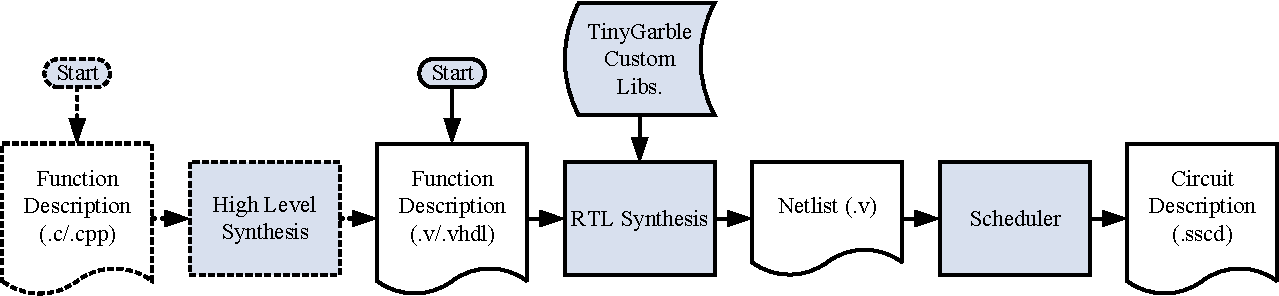
\includegraphics[width=0.95\textwidth]{synthesis_flow-crop.pdf}
\caption{TinyGarble GC synthesis flow.
  The inputs can be either a C/C++ program (translatable to HDL via a standard HLS tool) or a direct HDL description.
  The output is a scheduled circuit description ready to be garbled/evaluated.}
\label{fig:synthesis-flow}
\end{figure}

\begin{enumerate}
\item
  The input to TinyGarble GC synthesis is a file that describes a function written in an HDL like Verilog or VHDL.
  The function can also be written in a high level language like C/C++ and automatically translated to HDL using an HLS tool.

\item
  A standard HDL synthesis tool compiles the HDL to generate a netlist file.
  The synthesis tool optimizes the netlist based on the user defined objectives/constraints and a customized library.

\item
  The netlist is parsed and topologically sorted.
  Then, the sorted netlist is stored in fomat readable by TinyGarble GC engine.

\end{enumerate}

\begin{figure}[ht]
\centering
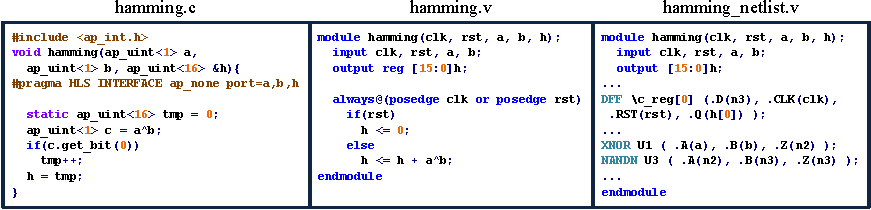
\includegraphics[width=\textwidth]{HLS_HDL_netlist-crop.pdf}
\caption{Sample files at the different steps of TinyGarble GC synthesis flow for Hamming distance function.}
\label{fig:globalflow_sample}
\end{figure}

\fig{fig:globalflow_sample} shows examples of files at different steps of TinyGarble GC synthesis flow for the Hamming distance function.
The \textsl{hamming.c} file contains the description of the function in the C language.
The user inputs this function to a HLS tool to generate the corresponding description in Verilog.
The resulting Verilog file is functionally similar to the \textsl{hamming.v} file shown in the figure, but it may look more complicated and be less efficient as it is generated by an automated tool.
A user can also write the description directly in Verilog to have more control on the circuit and therefore a more efficient netlist.
The \textsl{hamming.v} file is provided to an HDL synthesis tool along with the TinyGarble custom libraries to generate netlist \textsl{hamming\_netlist.v}.
The netlist describes the same function as \textsl{hamming.c} and \textsl{hamming.v} but uses the logic cells provided in the technology library.
The technology library contains 2-input-1-output logic cells to be compatible with TinyGarble GC engine.

In the following, we describe the details of the synthesis steps and how we manipulate the synthesis tools in each of the steps to generate optimized netlists for the GC protocol.

\subsection{Synthesis library}
The first step in the synthesis flow is to convert arithmetic and conditional operations like add, multiply, and if-else to their logical representations that fits best to the user's constraints.
For example, the sum of two N-bit numbers can be replaced with an N-bit ripple carry adder in case of area optimization or an N-bit carry look ahead adder in case of timing optimization.
A library that consists of these various implementations is called a \emph{synthesis library}.
We develop our own synthesis library that includes implementations customized for the GC protocl.
In this library, we build the arithmetic operations based on a full adder with one AND gate \cite{boyar2006concrete} and conditional operations based on a 2-to-1 multiplexer (MUX) with one AND gate \cite{kolesnikov2008improved}.

\subsection{Technology library}\label{sect:syn-tech}
The next step is to map the structural representation onto a \emph{technology library} to generate the netlist.
A technology library contains basic units available in the target platform.
For example, tools targeting Field Programmable Gate Arrays (FPGAs) like Xilinx ISE or Quartus contain Look-Up Tables and Flip Flops in their technology libraries, which form the architecture of an FPGA.
On the other hand, tools targeting Application Specific Integrated Circuits (ASICs) like Synopsys DC, Cadence, and ABC, may contain a more diverse collection of elements starting from basic gates like AND, OR, etc., to more complex units like FFs.
The technology library contains logical descriptions of these units along with performance parameters like their delay and area.
The goal of the synthesis tool in this step is to generate a netlist of library components that best fit the given constraints.
For HDL synthesis, we use tools targeting ASICs as they allow more flexibility in their input technology library.
We design a custom technology library that contains 2-input gates as they incur minimum garbled tables in the GC protocol compared to gates with more inputs.
We set the area of XOR gates to 0 and the area of AND gates to a non-0 value, e.g., 1.
By choosing area minimization as the only optimization goal, the synthesis tool produces a netlist with the minimum possible number of AND gates.
This reduces the total computation and communication of the GC protocol due to the Free-XOR optimization~\cite{kolesnikov2008improved}.

An additional feature of our custom technology library is that it contains non-standard gates (other than basic gates like NOT, AND, NAND, OR, NOR, XOR, and XNOR) to increase flexibility of mapping process.
For example, the logical functions $F = A\wedge B$ and $F = (\neg A)\wedge B$ requires equal effort in garbling/evaluation.
However by using only standard gates, the second function will require two gates (a NOT gate and an AND gate) and store one extra pair of keys for $\neg A$ in the memory.
We include four such non-standard gates with an inverted input in our custom library.
XOR, XNOR, and NOT gates are free so their area is set to 0.
The area of the rest of gates, similar to the area of AND, is set 1.
In order to be consist with the previous work in the literature, we use ``number of AND gates'' to refer to the number of non-free gates in a circuit throughout this thesis.
Due to the Free-XOR optimization, this metric directly corresponds to time and communication cost of garbling/evaluating the circuit.

\section{Offline Circuit Synthesis}
In TinyGarble GC synthesis, we use HDL synthesis tools in an offline manner to generate a circuit for a given functionality.
This offline synthesis followed by a topological sort provides a ready-to-use circuit description for any GC implementations including our TinyGarble GC engine.
This approach, unlike online circuit generation, does not require misspending time for circuit generation during garbling/evaluation.
It also enables the use of beneficial synthesis optimization techniques that were previously infeasible for online generation.
Moreover, the synthesis tools have a global view of the circuit, unlike previous work that manually optimized small modules of the circuit.
This allows more effective optimization for any arbitrary function and set of constraints.

\section{Limitation}\label{sect:syn-limit}
The synthesis approach has certain limitations when it comes to generating combinational circuits for extremely large functions.
The amount of memory and computation resources required by HDL synthesis tools considerably increase for generating large combinational circuits.
Generally, synthesis tools are not designed to support such large scale combination circuits.
This means HDL synthesis for GC cannot be scaled, at least automatically, for large functions using current setting, i.e., synthesizing its combinational circuit.

However, most of these large functions include one or more recurring computation blocks (a.k.a, loops).
In combinational representation, these loops have to be unfolded and represented as repeated blocks in the circuits.
In hardware design, these functions are folded around their loops and are described using sequential circuits.
A sequential circuit has feedback loops and is evaluated for multiple times (sequential cycles), thus it is the most suited to represent the recurring blocks in large functions.
In the next chapter, we will discuss possibility of using sequential circuit for the GC protocol.
We will show how can we exploit loops in sequential circuits while the process of optimized circuit generation remains the same.
This allows us to befit from synthesis tools optimization even for large functions.
